\documentclass[10pt]{article}

\usepackage[margin=0.75in]{geometry}
\usepackage{amsmath,amsthm,amssymb}
\usepackage{xcolor}
\usepackage{cancel}
\usepackage{changepage}
\usepackage{tikz}
\usepackage{pgfplots}
\usepackage{physics}
\usepackage{minted}
\usepackage{hyperref}
\usepackage[inline]{enumitem}

\theoremstyle{definition}
\newtheorem{problem}{Problem}
\newtheorem{soln}{Solution}

\pgfplotsset{compat=newest}
\usetikzlibrary{lindenmayersystems}

\hypersetup{
    colorlinks=true,
    linkcolor=blue,
    filecolor=magenta,      
    urlcolor=cyan,
    pdftitle={Overleaf Example},
    pdfpagemode=FullScreen,
    }

\NewDocumentCommand{\evalat}{sO{\big}mm}{%
  \IfBooleanTF{#1}
   {\mleft. #3 \mright|_{#4}}
   {#3#2|_{#4}}%
}

\tikzset{koch snowflake/.style={insert path={%
   l-system [l-system={rule set={F -> F-F++F-F}, axiom=F++F++F,
    step=3cm/3^#1, angle=60, order=#1,anchor=center}] -- cycle}}}

\title{Calculus II: Assignment 7}
\author{Jeremy Favro}
\date{\today}

\begin{document}

\maketitle

\noindent A shape that looks something like a snowflake is defined by the following process:\\

\begin{adjustwidth}{1cm}{1cm}
    \indent \indent \textit{Start with an equilateral triangle whose sides have length 1. If one modifies
        each of the line segments composing the triangle by cutting out the middle third
        of the segment, and then inserting an outward-pointing “tooth,” both of whose
        sides are as long as the removed third, one gets a six-pointed star. Suppose one
        repeats this process for each of the line segments making up the star, then to
        each of the line segments making up the resulting figure, and so on. The first
        few steps are illustrated below:}
    \footnote{Thank you to the creators of the \href{https://tikz.dev/library-lsystems}{lindenmayersystems} TikZ library for making drawing the fractals here a lot easier}
    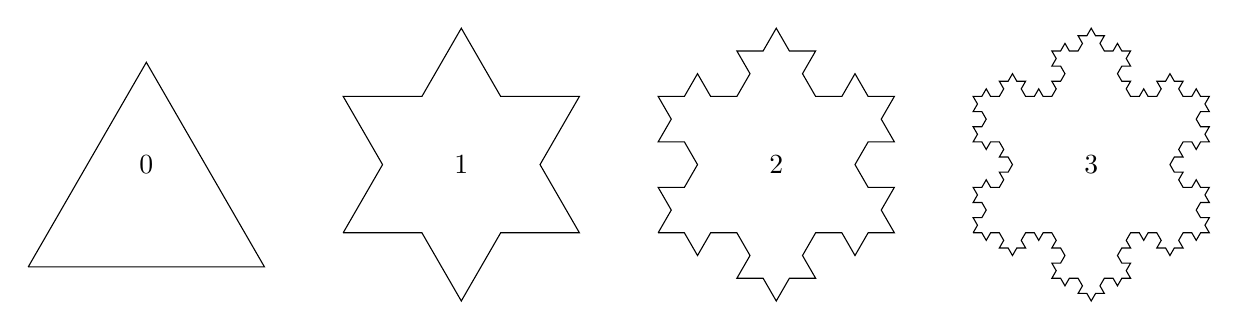
\begin{tikzpicture}
        \foreach \i in {0,...,3}
        \draw ({\i+\i*3},0) [koch snowflake=\i] node [text=black, font=\rm] {\i};
    \end{tikzpicture}
\end{adjustwidth}
\noindent The snowflake shape is the limit of this process; \emph{i.e.} what you have after infinitely many steps.\\

% PROBLEM 1
\begin{problem}
What is the length of the perimeter of the snowflake shape?
\end{problem}
\begin{soln}
    We know that for every step, we remove a third of the length of each side then add it back plus another third (adding $\frac{1}{3}$ the length of each side each step).
    So at step one we remove a third of the length of each side, then add them back plus a third, meaning we added in total $3\cdot\frac{1}{3}$ side lengths,
    at step two we remove a third of a third of the original side length from all sides in step one then add it back plus another third of a third,
    meaning we added $12\cdot\frac{1}{9}$ side lengths. In the third step we removed a third of a third of a third from each side, added it back plus
    another third of a third of a third, meaning we added in total $36\cdot\frac{1}{27}$ side lengths.\\

    There's a few patterns that emerge here. First of all, and probably easiest to notice is that at each step we multiply the number of sides by 4,
    starting from 3 (we have $3\cdot 4^{n_{step}}$ sides at any given $n_{step}$). Secondly, because we add $\frac{1}{3}$ the length of each side at each step,
    we end up with an individual side length of $\frac{1}{3^{n_{step}}}$ for any given $n_{step}$.

    Knowing that the perimeter is just the length of each side times the number of sides for a region with sides of equal length, we can now easily determine a general equation for the perimeter.
    $l_{side}(n_{step})=\frac{1}{3^{n_{step}}}$ and $n_{sides}(n_{step})=3\cdot 4^{n_{step}}$. So $p({n_{step}})$ is:

    \begin{align*}
         & = \frac{1}{3^{n_{step}}} \cdot 3\cdot 4^{n_{step}} \\
         & = 3\left(\frac{4}{3}\right)^{n_{step}}
    \end{align*}
    \noindent And as $n_{step}\to \infty, \, \lim_{n_{step} \to \infty} = 3\left(\frac{4}{3}\right)^{n_{step}}=\infty$, using $\lim_{x \to \infty} c^x=$ $\begin{cases}
            0      & |c|< 1 \\
            1      & |c|= 1 \\
            \infty & |c|> 1
        \end{cases}$
    \begin{center}
        $\therefore$ The perimeter of the snowflake is infinite.
    \end{center}
\end{soln}

% PROBLEM 2
\begin{problem}
What is the area of the snowflake shape?
\end{problem}
\begin{soln}
    At step 0, the area is $\frac{\sqrt{3}}{4}$, which is the area of an equilateral triangle with side length 1. In step 1 we add 3 equilateral triangles of side length $\frac{1}{3}$, so the area added is
    $3\cdot\frac{\sqrt{3}}{4}\cdot\frac{1}{3^2}$. In the second step we add 12 equilateral triangles of side length $\frac{1}{9}$, making the area added $12\cdot\frac{\sqrt{3}}{4}\cdot\frac{1}{9^2}$.\\

    As with question 1 there are two important patterns emerging here. The number of triangles added at any given $n_{step}$ is $3\cdot 4^{n_{step}-1}$, and the area of each of these triangles is
    $\frac{1}{3^{2n_{step}}}\cdot\frac{\sqrt{3}}{4}$. Multiplying the area of one triangle by the number of triangles at $n_{step}$ will give the area added at $n_{step}$, so the general formula for the
    area added at any $n_{step}$ is

    \begin{align*}
         & 3\cdot 4^{n_{step}-1}\cdot\frac{\sqrt{3}}{4}\cdot\frac{1}{3^{2n_{step}}}=\frac{4^{n_{step}-2}\sqrt{3}}{3^{2n_{step}-1}} \\
    \end{align*}
    \noindent which holds for all $n\geq0$, but I started out with a 0-indexed snowflake, so we'll just have to add the original area ($\frac{\sqrt{3}}{4}$) on to the sum. \\

    \noindent Summing the areas from 1 onwards yieldsw
    \begin{align*}
         & = \frac{\sqrt{3}}{4}+\sum_{n_{step}=1}^{\infty}\frac{4^{n_{step}-2}\sqrt{3}}{3^{2n_{step}-1}}                                                                          \\
         & = \frac{\sqrt{3}}{4}+\sum_{n_{step}=1}^{\infty}\frac{4^{n_{step}-2}\sqrt{3}}{9^{n_{step}-1}} \rightsquigarrow \text{ sum identity, } a=\frac{4^{1-2}\sqrt{3}}{9^{1-1}} \\
         & = \frac{\sqrt{3}}{4}+\frac{\frac{\sqrt{3}}{12}}{1-\frac{4}{9}}                                                                                                         \\
         & = \frac{\sqrt{3}}{4}+\frac{3\sqrt{3}}{20}                                                                                                                              \\
         & = \frac{2\sqrt{3}}{5}                                                                                                                                                  \\
    \end{align*}

    \begin{center}
        $\therefore$ the area of the ``complete" snowflake is $\frac{2\sqrt{3}}{5}$
    \end{center}
    \noindent This answer seems a little paradoxical (infinite perimeter yet finite area) but I overheard a passing comment in lecture from Professor
    Bilaniuk that the final answer is a bit paradoxical, so it actually makes me a bit more confident to see the apparent paradox. It's also to my understanding that this is something that crops
    up in the real world when measuring the border length vs. area of countries, the more accurate the border measurement the closer it gets to infinity, which seems a little weird, but aligns with
    the result I'm seeing here, again making me a bit more confident.
\end{soln}
\end{document}